\documentclass[10pt, a4paper]{article}
\usepackage[left=1.5cm,text={18cm, 24cm},top={2cm}]{geometry}

\usepackage[czech]{babel}
\usepackage[utf8]{inputenc}
\usepackage[T1]{fontenc}

\usepackage{blindtext}
\usepackage{hyperref}
\usepackage{csquotes}
\usepackage{titling}

\usepackage{graphics}
\usepackage{picture}
\usepackage{epsf}
\usepackage{epstopdf}
\usepackage{pdflscape}

\usepackage{listings}
\usepackage{float} 


\begin{document}
\newcommand{\HRule}{\rule{\linewidth}{0.1mm}}

\begin{center}
	\textsc{\large Vysoké Učení Technické v Brně} \\[0.1cm]
			{\large Fakulta informačních technologií}\\
	\vspace{22px}
	\textsc{\Huge Signály a systémy} \\
	\huge Projekt\\
	\vspace{18px}
\end{center}
\large Jméno: Kateřina Mušková\\
\large Login: xmusko00\\
\large Datum: 10.12.2019\\
\HRule

\begin{flushleft}

\section{Věty}
	\begin{tabular}{l l}
		Název	&  Délka [s]\\ \hline
		sa1 & 4.00\\
    	sa2 & 3.03\\
    	si1943 & 4.85\\
    	si2107 &  2.73\\
    	si683 & 5.10\\
    	sx143 & 3.48\\
    	sx233 & 2.94\\
    	sx323 & 3.36\\
    	sx413 & 4.92\\
    	sx53 & 3.32\\
	\end{tabular}

\section{Klíčová slova}
	\begin{tabular}{l l}
		Název	&  Délka [s]\\ \hline
		q1 & 0.81\\
    	q2 & 0.76\\
	\end{tabular}

\section{Spektrogram}

\begin{figure}[h]
	\scalebox{0.8}{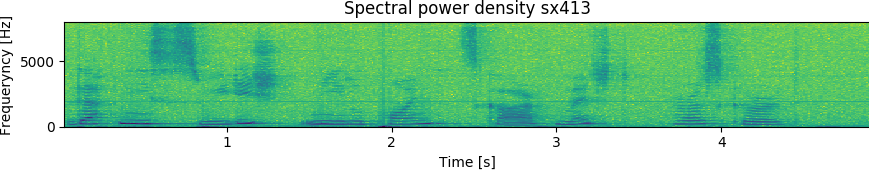
\includegraphics{img/sx413_desity.png}}
\end{figure}

\medskip
\section{Výpočet parametrů}

Jednoduše sečítám každých 16 koeficientu framu vykonnového spektra.
\begin{lstlisting}
def get_features(den_signal):
    # transpose
    switched = den_signal.transpose()

    # reshape  n x 256  => n x 16 x 16
    reshaped = np.reshape(switched, (len(switched), 16, 16))

    # cumpute sums, frames * 16
    features = np.array(list(row.sum() for frame in reshaped for row in frame))

    # reshape frames x 16
    features.resize((len(switched), 16))

    return features
\end{lstlisting}

Pokud bych však chtěla použít matici na každý frame, měla by ve sloupci k od pozice k*16 16 jedniček, jinak nuly.

\section{Skóre}
Výpočet skóre jsem také implemetovama podle zadání. Vzorec jsem rozdělila na 2 části: sentence\_probability a frame\_probability. Počítala jsem pouze každý 5. rámec.

\section{Grafický výstup}
\begin{figure}[H]
	\scalebox{0.6}{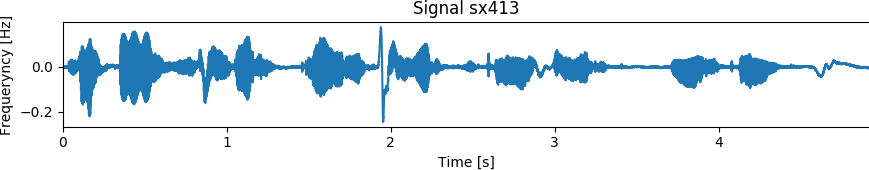
\includegraphics{img/sx413_signal.png}}\\
	\scalebox{0.6}{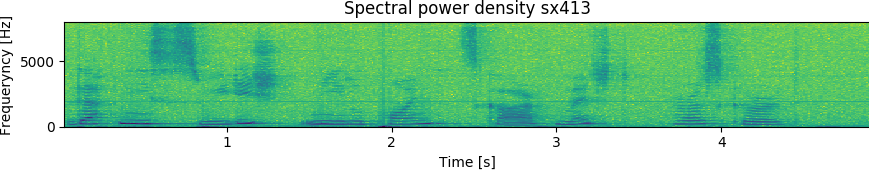
\includegraphics{img/sx413_desity.png}}\\
	\scalebox{0.6}{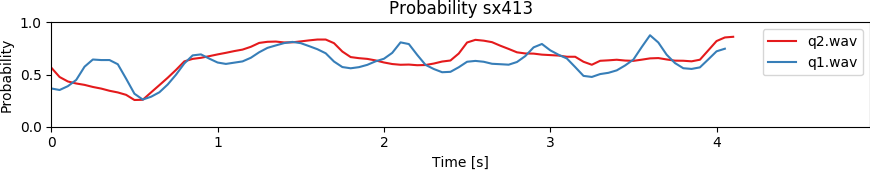
\includegraphics{img/sx413_probability.png}}\\
\end{figure}

\medskip

\begin{figure}[H]
	\scalebox{0.6}{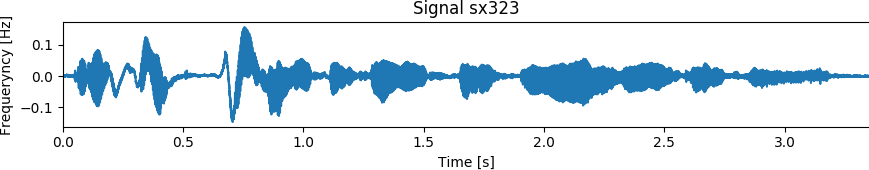
\includegraphics{img/sx323_signal.png}}\\
	\scalebox{0.6}{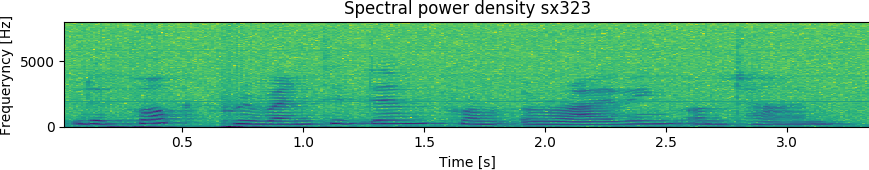
\includegraphics{img/sx323_desity.png}}\\
	\scalebox{0.6}{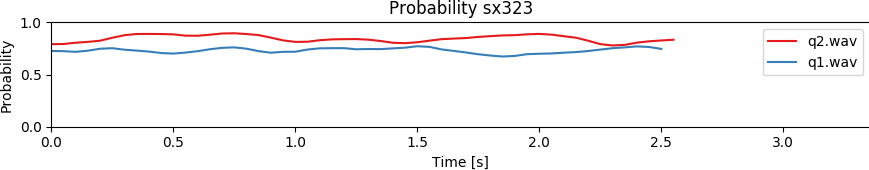
\includegraphics{img/sx323_probability.png}}\\
\end{figure}

\medskip

\begin{figure}[H]
	\scalebox{0.6}{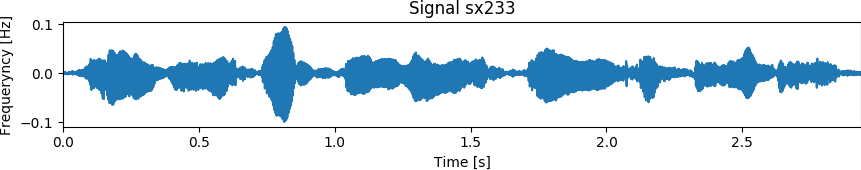
\includegraphics{img/sx233_signal.png}}\\
	\scalebox{0.6}{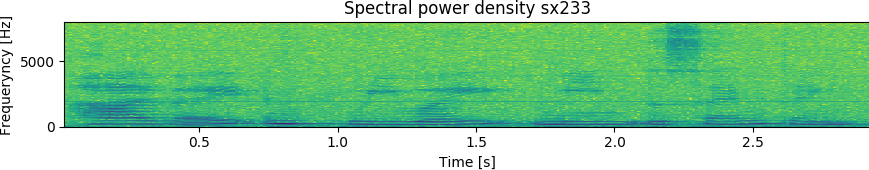
\includegraphics{img/sx233_desity.png}}\\
	\scalebox{0.6}{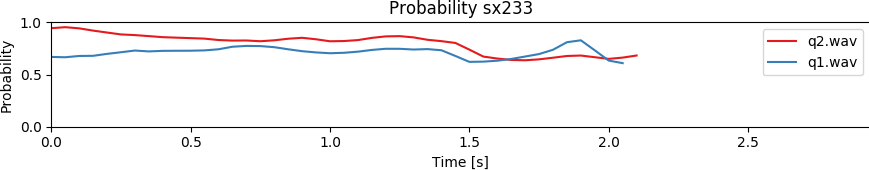
\includegraphics{img/sx233_probability.png}}\\
\end{figure}

\medskip

\begin{figure}[H]
	\scalebox{0.6}{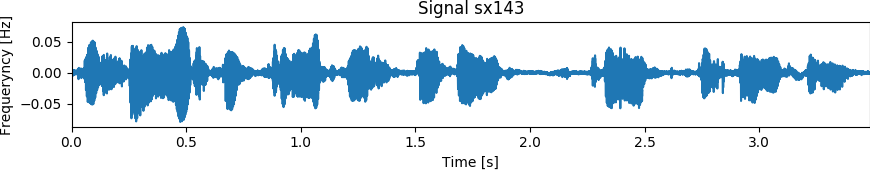
\includegraphics{img/sx143_signal.png}}\\
	\scalebox{0.6}{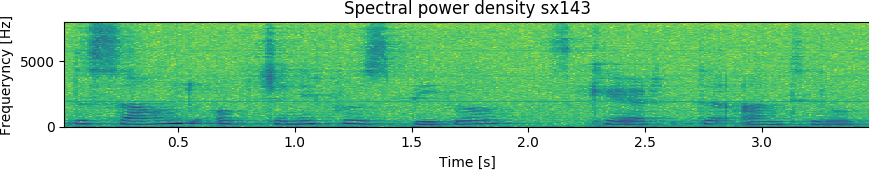
\includegraphics{img/sx143_desity.png}}\\
	\scalebox{0.6}{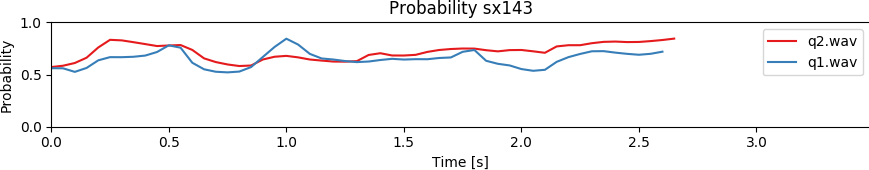
\includegraphics{img/sx143_probability.png}}\\
\end{figure}

\medskip

\begin{figure}[H]
	\scalebox{0.6}{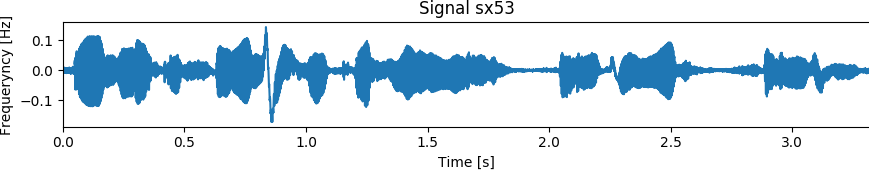
\includegraphics{img/sx53_signal.png}}\\
	\scalebox{0.6}{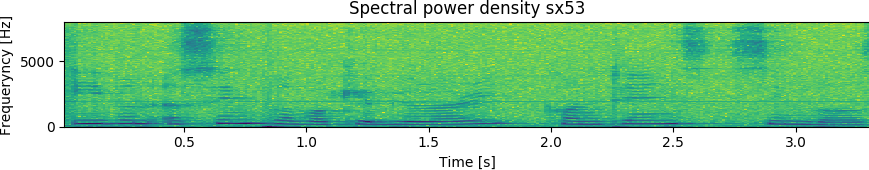
\includegraphics{img/sx53_desity.png}}\\
	\scalebox{0.6}{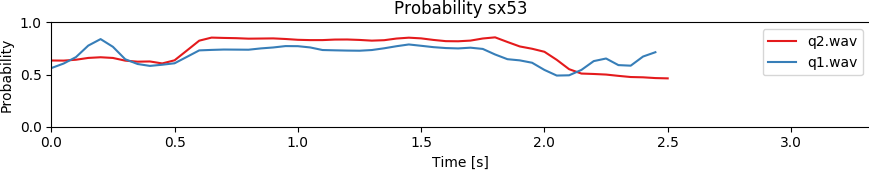
\includegraphics{img/sx53_probability.png}}\\
\end{figure}

\medskip

\begin{figure}[H]
	\scalebox{0.6}{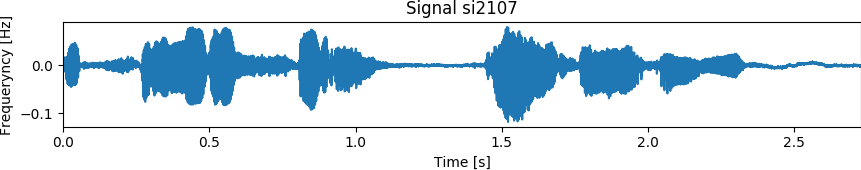
\includegraphics{img/si2107_signal.png}}\\
	\scalebox{0.6}{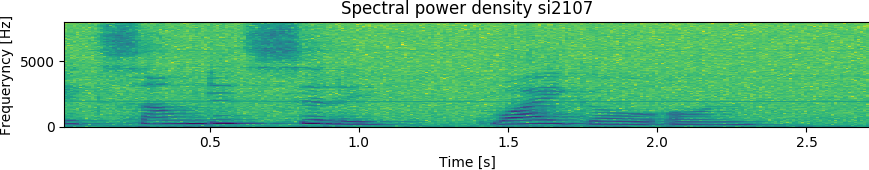
\includegraphics{img/si2107_desity.png}}\\
	\scalebox{0.6}{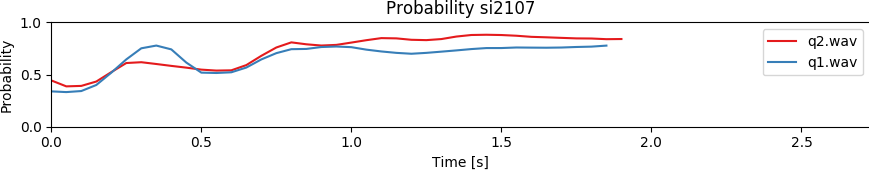
\includegraphics{img/si2107_probability.png}}\\
\end{figure}

\medskip

\begin{figure}[H]
	\scalebox{0.6}{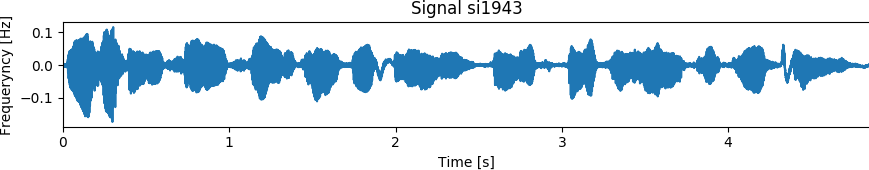
\includegraphics{img/si1943_signal.png}}\\
	\scalebox{0.6}{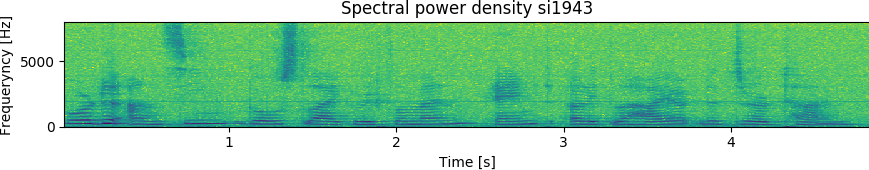
\includegraphics{img/si1943_desity.png}}\\
	\scalebox{0.6}{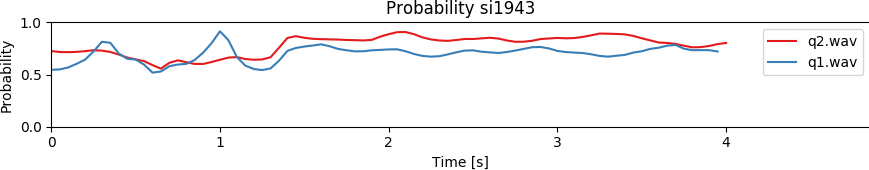
\includegraphics{img/si1943_probability.png}}\\
\end{figure}

\medskip

\begin{figure}[H]
	\scalebox{0.6}{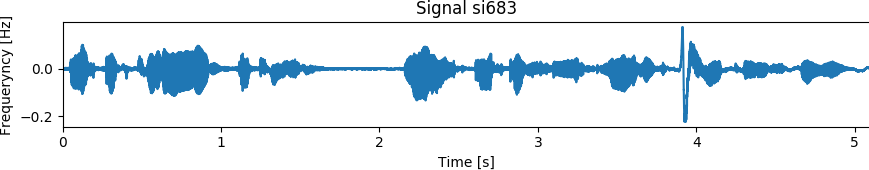
\includegraphics{img/si683_signal.png}}\\
	\scalebox{0.6}{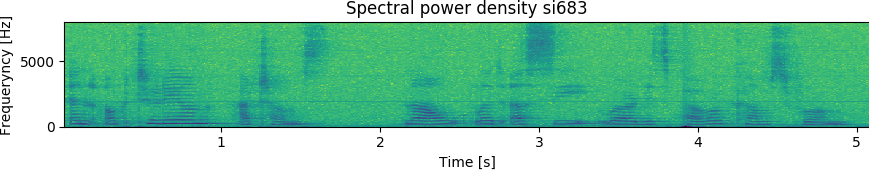
\includegraphics{img/si683_desity.png}}\\
	\scalebox{0.6}{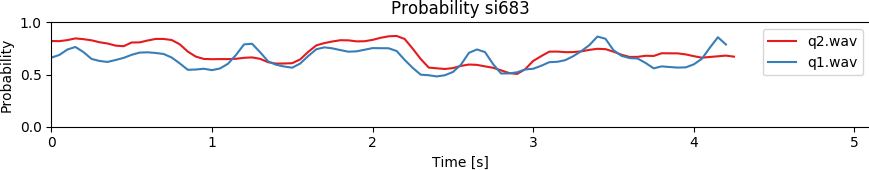
\includegraphics{img/si683_probability.png}}\\
\end{figure}

\medskip

\begin{figure}[H]
	\scalebox{0.6}{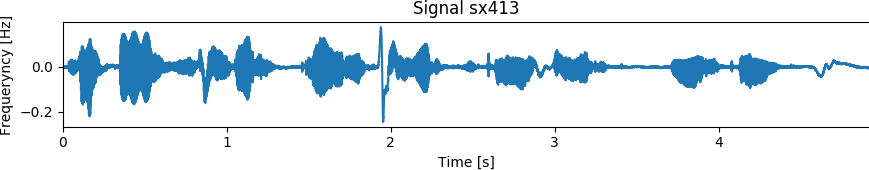
\includegraphics{img/sx413_signal.png}}\\
	\scalebox{0.6}{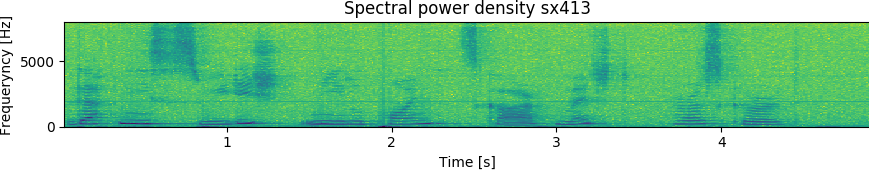
\includegraphics{img/sx413_desity.png}}\\
	\scalebox{0.6}{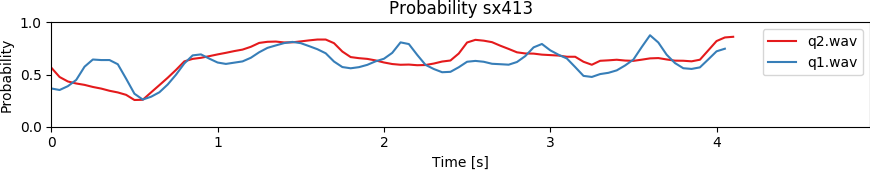
\includegraphics{img/sx413_probability.png}}\\
\end{figure}

\medskip

\begin{figure}[H]
	\scalebox{0.6}{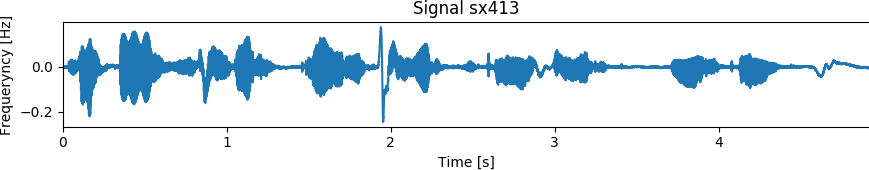
\includegraphics{img/sx413_signal.png}}\\
	\scalebox{0.6}{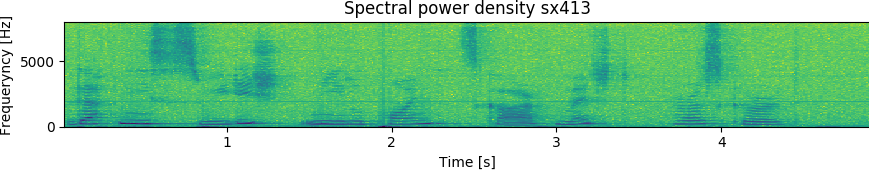
\includegraphics{img/sx413_desity.png}}\\
	\scalebox{0.6}{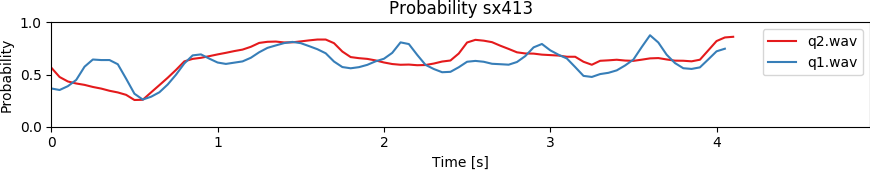
\includegraphics{img/sx413_probability.png}}\\
\end{figure}

\section{Práh}
Bohužel výsledky vyšly tak, že není možné určit žádný práh, který by byl schopný určit výskyt query.

\section{Výsledky}

\section{Závěr}
Detektor selhává.

\end{flushleft}
\end{document}



 
